%!TEX root = draft.tex
\section{Application to Stefan Problems}

We now propose an application of the level-set method on parallel adaptive cartesian mesh to the well studied stefan problem.

\subsection{Presentation of the problem}

We study the problem of the phase transition of a liquid melt to a solid crystaline structure. For a liquid melt and a solid crystal with respective heat capacities $c_l$ and $c_s$ and uniform thermal diffusivities $k_l$ and $k_s$, the respective temperatures $T_l$ and $T_s$ diffuse as

\begin{align*}
c_l \pd{T_l}{t} & = k_l \nabla T_l \quad \mathrm{in} ~~ \Omega^- , \\
c_s \pd{T_s}{t} & = k_s \Delta T_s \quad \mathrm{in} ~~ \Omega^+ .
\end{align*}

At the interface between the solid and the liquid phases, the temperature is defined as

\begin{equation*}
T_s = T_l = T_{\Gamma} = -\epsilon_c \kappa - \epsilon_v (\mathbf{V} \cdot \mathbf{n}),
\end{equation*}

where $\kappa$ is the local interface curvature, $V$ is the velocity of the interface, $\mathbf{n}$ is the outward normal to the solidification front and $\epsilon_c$ and $\epsilon_v$ are the curvature and kinetic undercooling coefficients. The velocity $V$ is defined from the jump in the heat flux at the interface

\begin{equation}
L (\mathbf{V} \cdot \mathbf{n}) = - \left[ k_l \pd{T_l}{\mathbf{n}} - k_s \pd{T_s}{\mathbf{n}} \right],
\end{equation}

with $L$ the latent heat.

\subsection{Scalability}

\subsection{Numerical experiments}

\begin{figure}[ht!]
\begin{center}
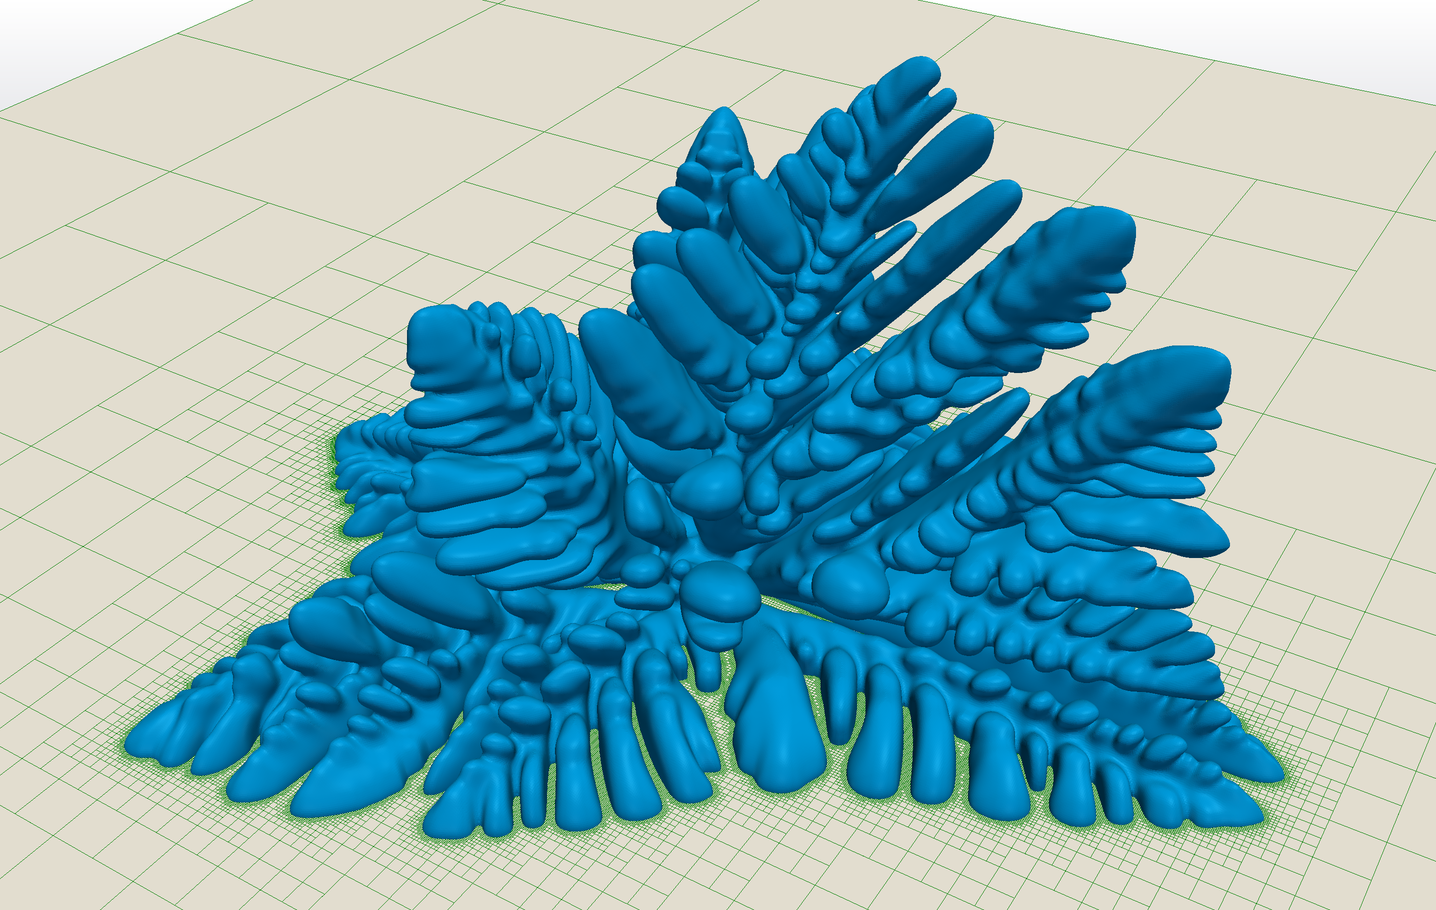
\includegraphics[width=.8\textwidth]{pictures/crystal_grid_low.png}
\end{center}
\end{figure}